% Sezione per illustrare il data path

\subsection{Data Path}
In Figura \ref{datapath} \`e mostrato il datapath; sono stati omessi i componenti utilizzati per il reset dei registri per favorire la leggibilit\`a.

Al fine di sfruttare al meglio la pipeline \`e stato suddiviso in 4 parti: 
\begin{itemize}
	\item Gestione indirizzi, per calcolare gli indirizzi di memoria cui accedere
	e mantenere un contatore;
	\item  Gestione input, per caricare nei registri i valori presenti in memoria;
	\item Analisi, per valutare l'appartenenza di un indirizzo a una WZ;
	\item Output, per gestire i segnali da inviare alla memoria.	
\end{itemize}

\subsubsection{Gestione degli indirizzi di memoria}

La gestione degli indirizzi cui accedere \`e realizzata con il registro \texttt{regnext} a 4 bit, che a inizio esecuzione viene inizializzato a 0 mentre alla memoria \`e richiesto l'indirizzo da codificare. In seguito, il registro inizia un ciclo di conteggio per poter accedere a tutte le celle di memoria contenenti gli indirizzi delle Working Zones e mantenere un contatore utile a gestire gli offset dati dalla pipeline.

Questo modulo \`e realizzato in VHDL con un process per realizzare \texttt{regnext} (compreso il sommatore collegato) e due costrutti \texttt{with/select} per i multiplexer in serie. Il valore di \texttt{o\_address} viene infine ricavato concatenando i dodici zeri meno significativi all'uscita dei multiplexer (per raggiungere i 16 bit degli indirizzi).

\subsubsection{Gestione degli input}

Per gestire i valori di input sono utilizzati due registri a 8 bit collegati a \texttt{i\_data}; il registro \texttt{regin} contiene l'indirizzo da codificare, mentre \texttt{regwz} l'indirizzo base della Working Zone in esame in questa fase (il cui numero corrisponde a \texttt{regnext}$ - 1$ per l'offset di pipeline).

La realizzazione in VHDL si compone semplicemente di due registri (realizzati con dei process) collegati all'input e attivati mai contemporaneamente.

\subsubsection{Analisi}
La fase di analisi si avvale infine del registro \texttt{regsub} a 8 bit (inizializzato a un valore arbitrario non significativo), che contiene la differenza tra l'indirizzo da codificare e l'indirizzo base della WZ; se questo valore \`e compreso o uguale tra 0 e 3 allora l'indirizzo fa parte della WZ e viene attivato il flag \texttt{is\_in} (che blocca il caricamento dei registri \texttt{regnext} e \texttt{regsub} per congelare il sistema).

Il codice di realizzazione si avvale di un process per calcolare e salvare il valore di \texttt{regsub}, e di una batteria di comparatori per determinare il valore di \texttt{is\_in}, ottenuto in modo combinatorio con un'espressione logica.

\subsubsection{Output}
Da un punto di vista di pipeline la fase di output pu\`o essere considerata unita a quella di analisi, poich\'e composta solo da reti combinatorie (si trovano quindi sulla stessa Working Zone). Utilizzando il valore di \texttt{is\_in} vengono selezionati i 7 bit meno significativi dell'output:
\begin{itemize}
	\item Se \texttt{is\_in} = 0, viene selezionato il valore di \texttt{regin};
	\item Se \texttt{is\_in} = 1, l'uscita risulta essere la concatenazione della WZ e della codifica one-hot del valore di \texttt{regsub}.
\end{itemize}
In quest'ultimo caso, il valore della Working Zone in uscita \`e determinato come i 3 bit meno significativi del valore (bloccato da \texttt{is\_in}) contenuto in \texttt{regnext}, cui viene sottratto l'offset dovuto al ritardo nella pipeline (ovvero 2 + 1 dovuto alla commutazione di \texttt{regnext}); la WZ \`e quindi \texttt{regnext}$ - 3$. Inoltre, \texttt{is\_in} stesso viene utilizzato come bit pi\`u significativo dell'output.
\begin{figure}[t]
	\centering	
	{\includegraphics[scale=0.7,keepaspectratio]
		{1hot.eps}}
	\caption{Encoder one-hot a due ingressi}
	\label{1hot} 
\end{figure}
La codifica one-hot a 2 ingressi \`e invece ottenuta attraverso una rete combinatoria (Illustrata in Figura \ref{1hot}) ricavata dalla seguente tavola di verit\`a:
\begin{center}
	\begin{tabular}{c c|c c c c}
		A & B & U3 & U2 & U1 & U0 \\
		\hline
		0 & 0 & 0 & 0 & 0 & 1 \\
		0 & 1 & 0 & 0 & 1 & 0 \\
		1 & 0 & 0 & 1 & 0 & 0 \\
		1 & 1 & 1 & 0 & 0 & 0
	\end{tabular}
\end{center}

La codifica VHDL del modulo viene realizzata con un costrutto \texttt{with/select} per il multiplexer (per cui uno degli ingressi risulta essere la concatenazione del valore della WZ attuale e dell'uscita dell'encoder one hot) e un'espressione logica per l'encoder one-hot.

